\documentclass[conference]{IEEEtran}
\IEEEoverridecommandlockouts
% The preceding line is only needed to identify funding in the first footnote.
% If that is unneeded, please comment it out.
\usepackage{cite}
\usepackage{amsmath,amssymb,amsfonts}
\usepackage{algorithmic}
\usepackage{graphicx}
\usepackage{textcomp}
\usepackage{xcolor}
\usepackage{url}
\def\BibTeX{{\rm B\kern-.05em{\sc i\kern-.025em b}\kern-.08em
    T\kern-.1667em\lower.7ex\hbox{E}\kern-.125emX}}
\begin{document}

\title{Agentic Python Dependency Resolution (APDR)}

\author{\IEEEauthorblockN{Danny Guan}
\IEEEauthorblockA{
\textit{Toronto Metropolitan University}\\
Toronto, Canada \\
d1guan@torontomu.ca}
\and
\IEEEauthorblockN{Karanvir Bhogal}
\IEEEauthorblockA{
\textit{Toronto Metropolitan University}\\
Toronto, Canada \\
karanvir.bhogal@torontomu.ca}
\and
\IEEEauthorblockN{Jamie}
\IEEEauthorblockA{
\textit{Toronto Metropolitan University}\\
Toronto, Canada \\
email address or ORCID}
}

\maketitle

\begin{abstract}
Python dependency resolution remains difficult when software artifacts omit, misstate, or fragment the metadata needed to reconstruct a runnable environment. Prior approaches have shown that neither purely static metadata recovery nor purely iterative repair is sufficient across the full range of Python dependency failures. This project proposes Agentic Python Dependency Resolution (APDR), a hybrid resolver that builds on SmartPip-style graph knowledge while extending it with cache-based evidence, heuristic package inference, optional large language model reasoning, and validation-guided recovery. APDR analyzes code snippets, infers likely Python versions and packages, pre-solves dependency constraints, validates candidate environments through execution, and uses failure feedback to revise later attempts. The resulting design aims to combine the structured search-space reduction of graph-based methods with the adaptability of execution-guided LLM-assisted repair.
\end{abstract}

\begin{IEEEkeywords}
Python dependency resolution, environment reconstruction, large language models, software configuration, agentic systems
\end{IEEEkeywords}

\section{Introduction}
Python dependencies remain difficult to reconstruct because the Python ecosystem contains a large and evolving collection of packages, versions, aliases, and transitive constraints. Even when source code is correct, programs can still fail because of missing packages, unsupported interpreter versions, renamed imports, or incomplete configuration metadata. These problems appear especially often in older repositories and in code snippets where dependency information is absent or unreliable. Traditional dependency-management methods struggle in such settings because they assume that environment descriptions are explicit and trustworthy, which is frequently not the case.

Recent work has explored whether large language models can help address this problem. Bartlett, Liem, and Panichella introduced PLLM, a retrieval-augmented framework that identifies likely dependencies, retrieves package and version information, validates candidate environments, and then repairs failures using execution feedback \cite{b5}. PLLM improves substantially over earlier baselines, but structured systems such as PyEGo and smartPip still provide valuable information about package relationships, aliasing, and compatibility constraints \cite{b3,b4}. These observations suggest that dependency resolution should not rely on a single pathway. Instead, effective systems should combine multiple weak but complementary signals, including imports, package metadata, graph-based knowledge, runtime error traces, and prior failed attempts.

This project adopts that hybrid perspective through Agentic Python Dependency Resolution (APDR). APDR builds on SmartPip-compatible dependency knowledge rather than replacing it. SmartPip provides graph-based information about package relationships, versions, and constraints, while APDR adds a coordinating resolution layer that combines cached evidence, heuristic and LLM-assisted package inference, and validation-driven recovery. In this design, APDR uses structured dependency knowledge to narrow the search space and then extends that knowledge with execution-based feedback to select dependency sets that are not only plausible statically, but runnable in practice.

\section{Background and Related Work}
Environment dependency inference seeks to recover the third-party packages, interpreter version, and auxiliary runtime requirements needed to execute a Python program. This task becomes difficult when declarative metadata such as \texttt{requirements.txt} or \texttt{pyproject.toml} is missing, incomplete, or inconsistent with the code. Prior empirical work showed that this problem is widespread: Horton and Parnin reported that many Python gists require non-trivial environment configuration, and their later DockerizeMe system demonstrated that graph-based inference can recover missing dependencies for such snippets \cite{b1,b2}.

Subsequent work explored complementary forms of reasoning. PyEGo formulates environment dependency inference as a knowledge-graph problem over packages, Python interpreters, and system libraries, and then solves constraints over a program-specific subgraph \cite{b3}. smartPip similarly exploits a pre-built dependency knowledge base and SMT-based reasoning to prune the search space and resolve dependency conflicts more efficiently \cite{b4}. In contrast, PLLM treats dependency repair as an iterative, retrieval-augmented, and execution-guided process in which an LLM proposes candidate environments, observes validation feedback, and refines later attempts \cite{b5}. Reported results show that this strategy outperforms both PyEGo and ReadPyE on HG2.9K \cite{b5}.

APDR positions itself as a hybrid extension of this line of work. Rather than choosing between symbolic dependency knowledge and agentic repair, APDR integrates both within a staged resolver. APDR first analyzes each snippet directly by extracting imports, scanning nearby configuration files, and inferring a plausible Python version window. APDR then resolves candidate packages through multiple evidence sources, including cached import mappings, previously validated solutions, heuristic alias and package-family rules, SmartPip-compatible KGraph metadata, and optional LLM-based import resolution when ambiguity remains. After APDR constructs an initial dependency set, it expands transitive requirements, pre-solves version constraints to produce a candidate environment, and validates that environment through isolated execution. When validation fails, APDR classifies the failure, applies deterministic recovery rules or LLM-guided corrections, and iterates on the dependency set. In this way, APDR extends the structured reasoning emphasized by smartPip and PyEGo with the execution-driven adaptivity demonstrated by PLLM.

\section{Approach}
We organize APDR as five functional stages: entry, resolution, knowledge, validation, and outputs. Rather than assigning Python dependency resolution to a single model or fixed rule set, APDR distributes the task across stages that contribute different forms of evidence and decision-making. The entry stage standardizes benchmark execution, the resolution stage identifies candidate packages and versions, the knowledge stage provides static and learned evidence, the validation stage tests candidate environments and guides recovery, and the output stage records both final artifacts and diagnostic traces.

At the entry stage, APDR receives benchmark cases from the hard-gists dataset through a compatibility wrapper that invokes the APDR command-line interface and standardizes execution, artifact generation, and evaluation across cases. The resolution stage begins by parsing each snippet, extracting imports, scanning nearby configuration files, and inferring a plausible Python version range from the code. Before running the full resolver, APDR also short-circuits cases that depend on unavailable host runtimes or that match previously learned unsolvable patterns.

For the remaining cases, APDR applies a tiered resolution strategy. It first reuses fast-path cache entries, including learned import-to-package mappings and previously validated solutions for identical import sets. It then applies heuristic matching and curated package-family knowledge to handle exact package-name matches, aliases, deprecated names, and common namespace conflicts. When unresolved imports remain and LLM support is enabled, APDR invokes an Ollama-backed LLM to assess solvability, map ambiguous imports to candidate PyPI packages, and suggest versions for unresolved cases.

The knowledge stage combines repository-provided resources with information learned during previous runs. APDR loads seed mappings, alias tables, dependency-family knowledge, and Python standard-library lists from the repository, and it augments these with file-backed caches that store learned import mappings, version constraints, lockfiles, build artifacts, failure patterns, unsolvable modules, and validated environments. For package versions and dependency specifications, APDR queries cached metadata first, then consults SmartPip-compatible KGraph and SMTpip data, and finally falls back to PyPI when necessary.

After APDR selects candidate packages, it expands transitive dependencies and runs a pre-solve step over version constraints to construct a candidate \texttt{requirements.txt}. The validation stage then tests this candidate environment by creating isolated local Python environments by default, installing the proposed dependencies, and running smoke tests or snippet execution. Optional Docker and LLM-assisted validation backends are also available. If validation fails, APDR analyzes the logs, classifies the failure, applies deterministic recovery rules or LLM-guided package corrections, and retries within a bounded budget. Finally, the output stage records the resolved requirements, the resolution report, per-case metadata files, per-attempt logs, solver snapshots, iteration artifacts, and optional benchmark-context and LLM-trace files.

\begin{figure*}[t]
\centering
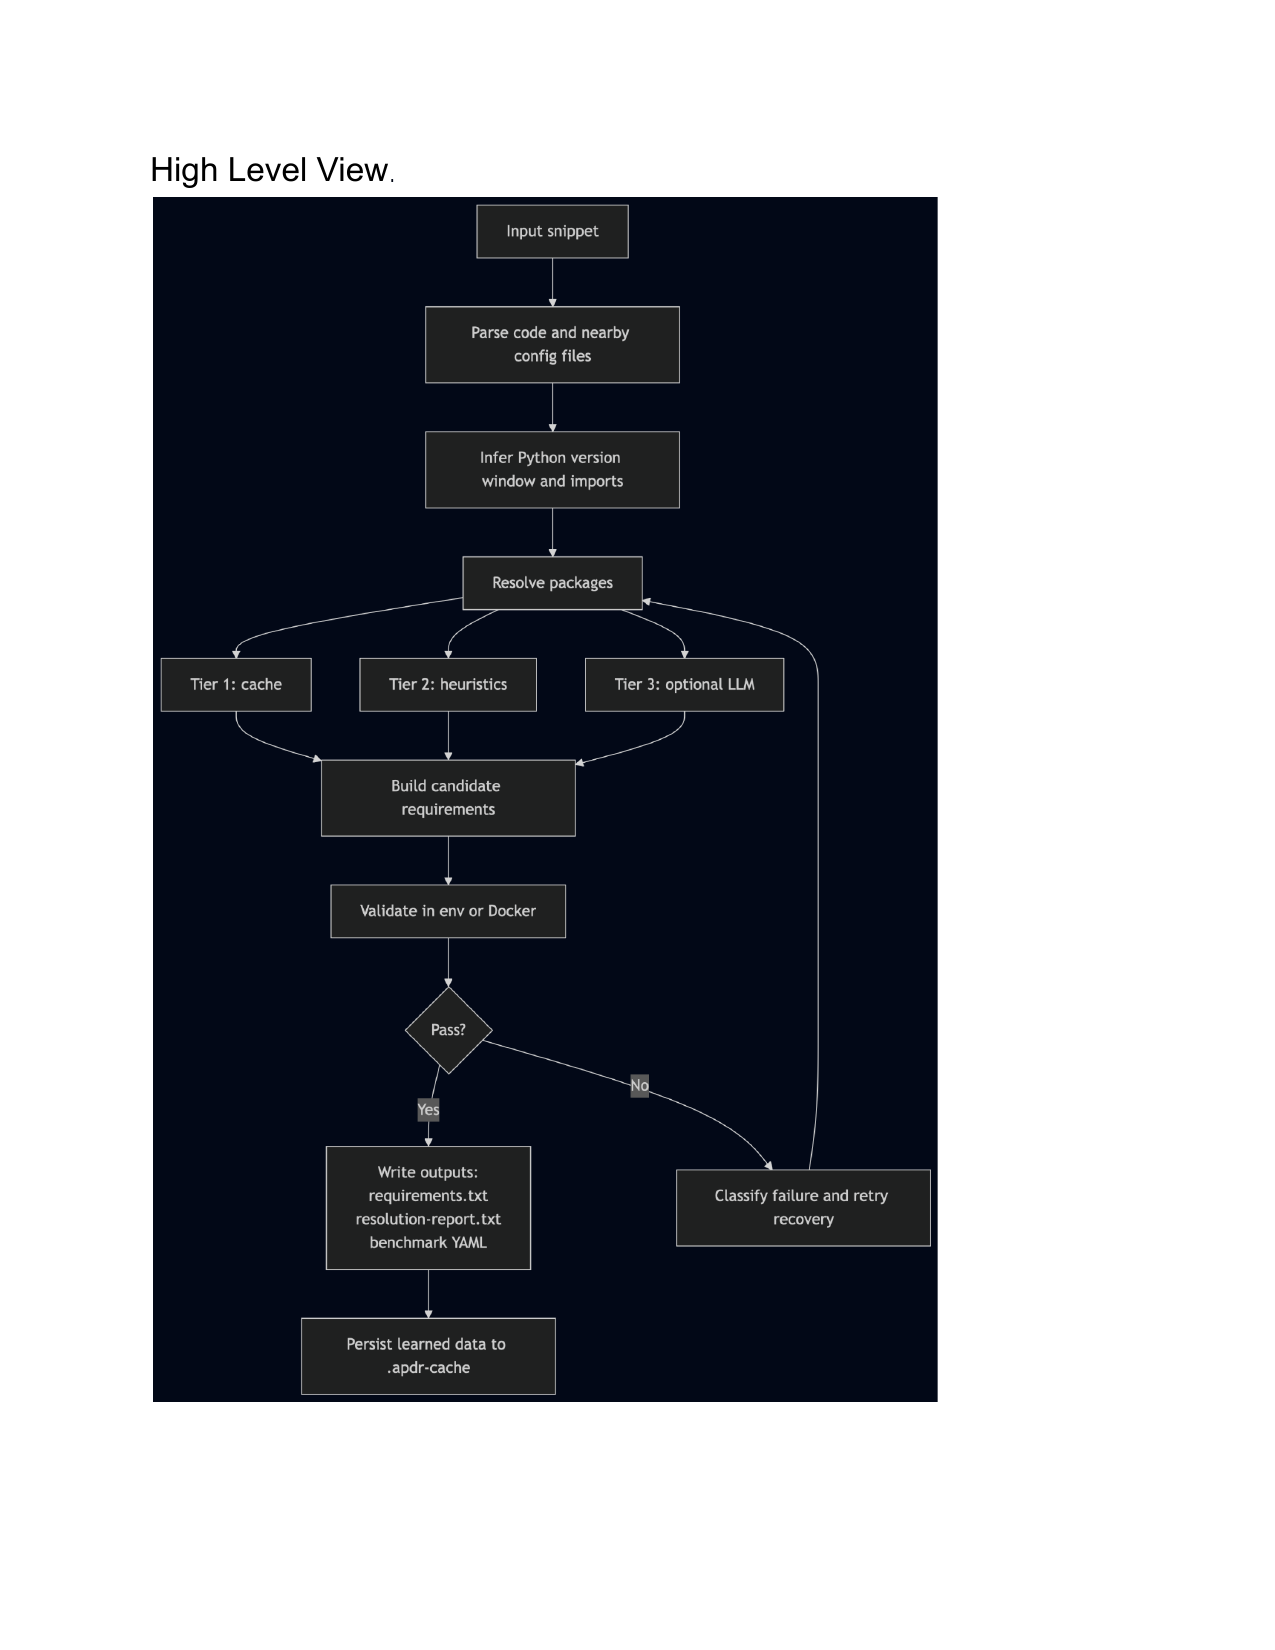
\includegraphics[width=0.78\textwidth]{figures/apdr-high-level-view.png}
\caption{High-level APDR workflow incorporated from the project proposal.}
\label{fig:apdr-high-level}
\end{figure*}

\begin{figure*}[t]
\centering
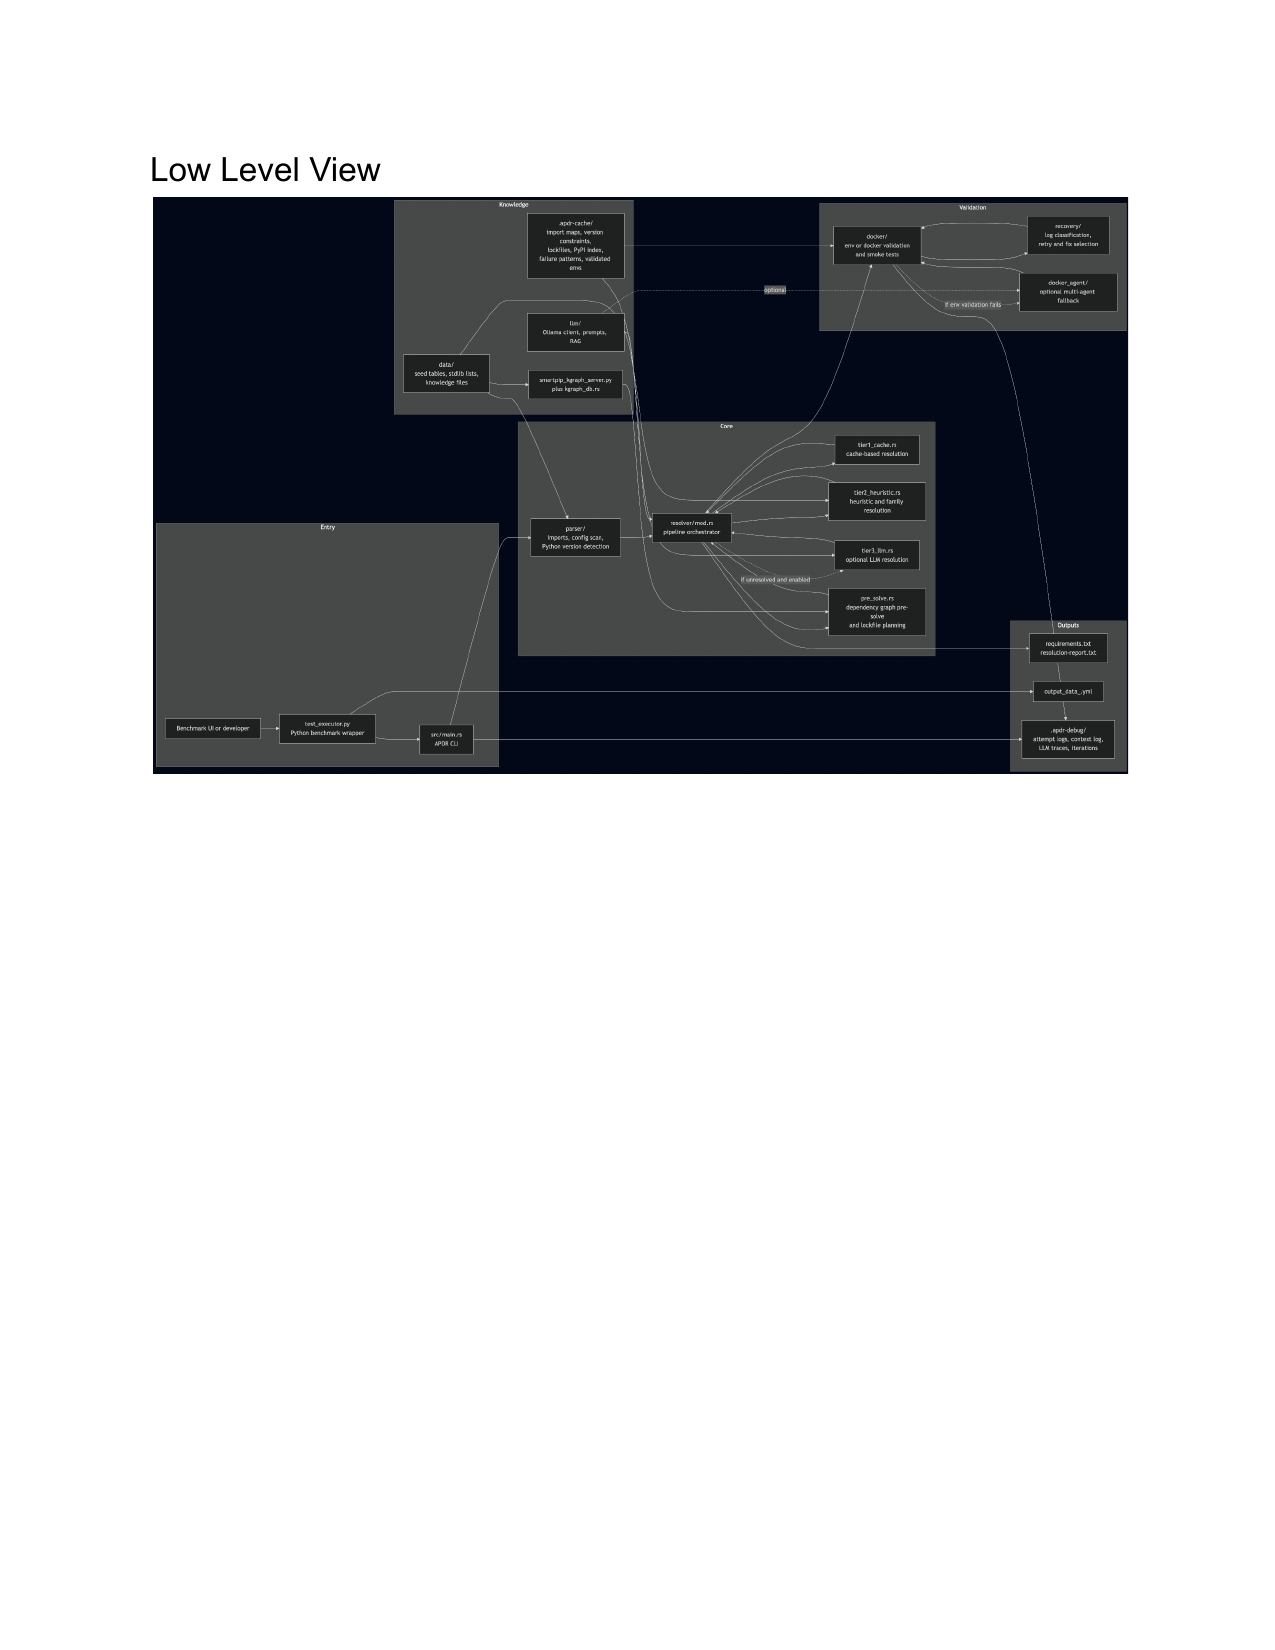
\includegraphics[width=\textwidth]{figures/apdr-low-level-view.png}
\caption{Low-level APDR architecture view incorporated from the project proposal.}
\label{fig:apdr-low-level}
\end{figure*}

\section{Performance Considerations}
APDR is designed not only to improve dependency resolution quality, but also to keep the runtime cost of that process manageable. One important design choice is that APDR orders its resolution stages from cheapest to most expensive. Fast cache lookups and heuristic matching run before any optional LLM calls, which allows many straightforward cases to be resolved without paying the overhead of iterative model inference. APDR also exits early for snippets that match known unsolvable patterns or that clearly depend on unavailable host runtimes. These fast paths reduce wasted work and help reserve more expensive validation and recovery steps for genuinely ambiguous cases.

The implementation also includes several optimizations aimed at reducing metadata lookup cost. APDR uses SmartPip-compatible KGraph data as a high-value source of package-version and dependency information, and it prefers native SQLite-based KGraph queries over slower subprocess-based lookups whenever possible. During pre-solving, APDR bulk-prefetches direct-package metadata from KGraph before exploring version assignments, which reduces repeated lookup overhead later in the solve. In addition, the in-process knowledge cache is populated on demand rather than fully loaded at startup, which lowers both startup time and memory pressure for cases that only touch a small part of the overall package graph.

Parallelism is another important part of APDR's performance strategy. When multiple candidate Python versions must be considered, APDR can solve across those candidates in parallel rather than exploring them one at a time. This allows the resolver to search several plausible interpreter configurations simultaneously and stop early once one candidate produces a satisfiable solution. Validation cost is also controlled through reuse and bounded execution. APDR caches previously validated environments, reuses wheel downloads through a wheelhouse cache, and enforces an overall validation budget so that repeated retries do not expand without limit. In high-confidence cases, APDR can even skip full validation once it has both a satisfiable pre-solve result and sufficiently strong confidence scores across the selected dependencies. Together, these choices make APDR's hybrid pipeline more practical by improving throughput while still preserving the benefits of validation-guided recovery.

\section{Experimental Setup}
The planned evaluation uses the benchmark harness provided with the project repository and the hard-gists workload associated with HG2.9K-style dependency-resolution cases. APDR will be run through its benchmark wrapper so that each case follows a consistent pipeline for parsing, resolution, validation, and artifact collection. When LLM support is enabled, APDR will use an Ollama-hosted model for package-resolution and recovery steps. The evaluation will compare APDR against available baselines and historical benchmark data, including PLLM and other reported systems in the repository.

We plan to evaluate APDR using three main criteria: resolution success rate, time required per case, and the quality of the produced runnable environments. We will also examine how often APDR succeeds through cache reuse, heuristic resolution, LLM-assisted inference, and recovery after validation failure. This setup is intended to show not only whether APDR resolves more cases, but also which parts of the hybrid pipeline contribute most to successful outcomes.

\section{Empirical Results}
This section will report the empirical performance of APDR after the benchmark study is completed. In particular, it will compare APDR against baseline systems, summarize aggregate success rates and runtime costs, and analyze which failure categories remain difficult for the hybrid resolver. The final version will also discuss whether APDR's combination of graph-backed knowledge, cached evidence, and validation-guided repair improves robustness over single-strategy approaches.

\section{Threats to Validity}
Several threats to validity apply to this study. First, benchmark snippets may not fully capture the diversity of dependency failures seen in larger multi-file repositories. Second, LLM-assisted resolution may depend on the selected model, local serving configuration, and prompt design, which can affect reproducibility. Third, repository-provided caches and knowledge sources may advantage APDR on cases that resemble previously seen dependency patterns. Finally, successful validation in isolated environments does not always guarantee long-term maintainability or correctness in production settings. We include this section because these factors influence how broadly the reported results can be generalized.

\section{Conclusion and Future Work}
This project proposes APDR as a hybrid dependency-resolution framework that combines graph-based package knowledge, cache reuse, heuristic inference, optional LLM reasoning, and validation-guided recovery. The core idea is that difficult Python dependency problems should not be addressed through a single reasoning strategy alone. Instead, APDR coordinates multiple evidence sources to infer, test, and refine candidate environments. In future work, we plan to complete the empirical study, analyze the relative contribution of each resolution tier, and investigate stronger recovery strategies for cases involving legacy packages, host-runtime dependencies, and incomplete package metadata.

\begin{thebibliography}{00}
\bibitem{b1} E. Horton and C. Parnin, ``Gistable: Evaluating the executability of Python code snippets on GitHub,'' in \textit{2018 IEEE International Conference on Software Maintenance and Evolution (ICSME)}, 2018, pp. 217--227, doi: 10.1109/ICSME.2018.00031.

\bibitem{b2} E. Horton and C. Parnin, ``DockerizeMe: Automatic inference of environment dependencies for Python code snippets,'' in \textit{Proceedings of the 41st International Conference on Software Engineering (ICSE)}, 2019, pp. 328--338, doi: 10.1109/ICSE.2019.00047.

\bibitem{b3} H. Ye, W. Chen, W. Dou, G. Wu, and J. Wei, ``Knowledge-based environment dependency inference for Python programs,'' in \textit{Proceedings of the 44th International Conference on Software Engineering (ICSE)}, 2022, pp. 1245--1256, doi: 10.1145/3510003.3510127.

\bibitem{b4} C. Wang, R. Wu, H. Song, J. Shu, and G. Li, ``smartPip: A smart approach to resolving Python dependency conflict issues,'' in \textit{Proceedings of the 37th IEEE/ACM International Conference on Automated Software Engineering (ASE)}, 2022, doi: 10.1145/3551349.3560437.

\bibitem{b5} A. Bartlett, C. Liem, and A. Panichella, ``The last dependency crusade: Solving Python dependency conflicts with LLMs,'' in \textit{Proceedings of the 2025 40th IEEE/ACM International Conference on Automated Software Engineering Workshops (ASEW)}, 2025, pp. 66--73, doi: 10.1109/ASEW67777.2025.00022.
\end{thebibliography}

\end{document}
